\vspace{-0.5cm}
\section*{Task \#1: IST algorithm for solving LASSO}

\subsection*{Brief theoretical introduction}
When we have to solve an optimization problem, finding a \textit{simple approximate solution} is surely better than an exact but  
more complex one. 
In our case \textbf{simplicity} corresponds to \textbf{sparsity}. A solution is said to be \textbf{sparse} if it has \textbf{few non-zero elements}. A \textit{sparse optimization problem} can be formultated in the form $ \min_{x\in X} \  f(x) \ \text{s.t.} \ \Vert x \Vert_0 \le h$, where $x$ is the optimization variable and $f(x)$ the objective function. The main disadvantage of this formulation is the $\ell_0$-norm which, being \textit{non-convex and discontinuous}, makes the problem itself \textbf{hard} to be solved. Here the trick is the use of the $\ell_1$-norm as an approximation, which has better properties, first of all the \textbf{convexity}.\\
%Sparse Optimization is ubiquitous since the found solutions are easier to store and implement. Just to give an example, in machine learning one can find useful a \textbf{sparse model} with few parameters in order to avoid problems related to the overfitting (the model is too much linked to the training data).\\
In many real-world applications we need to find a \textbf{sparse solution} to a large underdetermined systems of linear equations. The presence of \textbf{measurement noise} in collecting data justify us in using a least-squares approach while the requirement on sparsity is fulfilled by introducing an $\ell_1$-based penalty. This raises the problem of \textbf{LASSO} (\textit{Least Absolute Shrinkage and Selection Operator}) defined as
\vspace{-0.2cm}
\begin{equation} \label{eq:LASSO} 
    x^* = \text{arg} \min_{x \in \mathbb{R}^n} \frac{1}{2}\Vert y-Ax \Vert_2^2 + \lambda \Vert x \Vert_1, \ \lambda >0
    \vspace{-0.2cm}
\end{equation}
where $\lambda$ is an hyperparameter to tune. There are many algorithms to solve the LASSO problem. However, the objective of this task is to analyze the \textbf{Iterative Shrinkage/Thresholding Algorithm} also called \textbf{ISTA}.

\vspace{-0.2cm}
\subsection*{Iterative Shrinkage/Thresholding Algorithm}
The algorithm on which we focus our attention is derived from the \underline{alternating minimization} of a \textit{surrogate funtional} $\mathcal{R}(x,b)$ which is obtained adding some terms to the one in (\ref{eq:LASSO}). 
\begin{algorithm}
    \caption{Iterative Shrinkage and Thresholding Algorithm (ISTA)} \label{alg:ISTA}

    \vspace{0.3cm}
    \begin{enumerate}   
        \itemsep-0.3em
        \item  \textsf{\textbf{Initialization}} $x_0 \in \mathbb{R}^n$, e.g. $x_0=0$
        \item \textsf{For each $k=0, ..., T_{max}$}
        \vspace{-0.5cm}
        \begin{equation*}
            x(k+1)=\mathbb{S}_{\lambda\tau}[x(k)+\tau A^T(y-Ax(k))], \quad 
            \mathbb{S}_{\lambda\tau}=
            \begin{cases}
                x_i-{\lambda\tau} & \text{if $x_i$>${\lambda\tau}$} \\
                x_i+{\lambda\tau} & \text{if $x_i$ < -${\lambda\tau}$}\\
                0 & \text{if $ \lvert x_i \rvert \le \alpha$}\\ 
            \end{cases}
        \end{equation*}
        \vspace{-0.7cm}
        \item \textbf{\textsf{Stop condition}}: $\Vert x(T+1) - x(T) \Vert < \delta,\ \delta=10^{-12}$
    \end{enumerate}
\end{algorithm}


\noindent
 $\mathbb{S}_{\lambda\tau}$ is the \textbf{Shrinkage/Thresholding operator}.
 The parameter $\lambda$ has a crucial role, in particular for $\lambda=0$ we just get the LS estimate of the full model, while for \textit{very large} $\lambda$ the LASSO estimates are exactly zero.
The \textbf{Algorithm (\ref{alg:ISTA})} has the following properties: (i) it is a \textbf{descent algorithm}, (ii) it converges to the minimum of LASSO; furthermore, its iterative nature makes it suitable for both \textbf{dynamic} and \textbf{distributed} settings.
\vspace{-0.2cm}
\subsection*{Analysis and Results}
In order to perform the analysis, data have been randomly generated: the entries of $C$ are distributed according $\mathcal{N}(0,1)$;  the entries of the (sparse) vector $x$ are assumed to be uniformly distributed; finally the solution is imposed to be 2-sparse. The \textbf{measurement phase} is distributed in the sense that the measurements have to be interpreted as taken by $q$ sensors, each one of them taking one measurement.
\subsubsection*{First aspect: Support recovery rate}
The \textbf{support} of a solution is the set of indexes at which the non-zero elements are placed. The analysis is performed on what is the \textbf{effect of increasing the number of sensors $q$} in the capability of the algorithm in recover correctly the support of the solution. To this aim, for each value of $q$ from 5 to 20, 20 experiments have been executed.
\begin{figure}[h]   
    \vspace{-1cm}
    \centering 
    \subfigure[Support recovery rate]
    {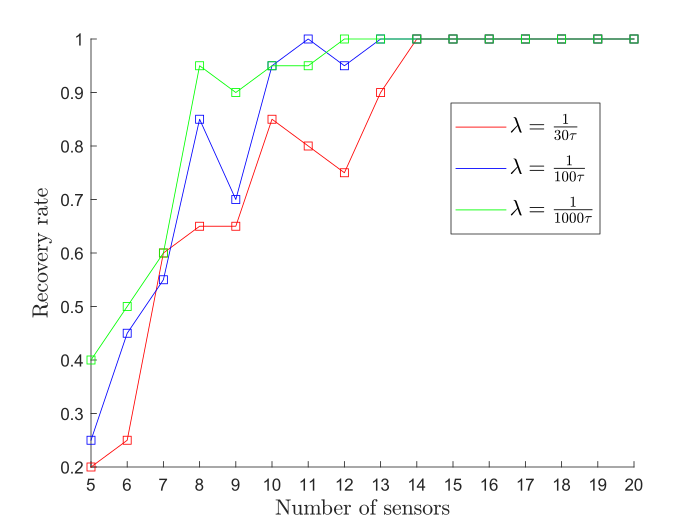
\includegraphics[scale=0.3]{img/SuppRecRate.png}}
    \subfigure[Convergency time (I)]
    {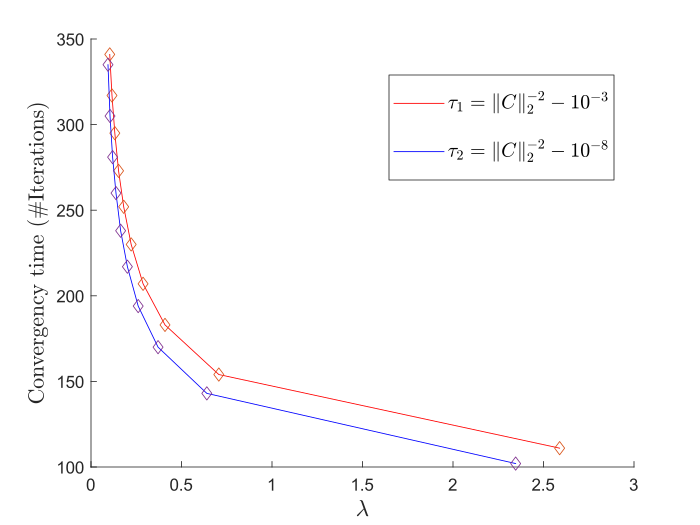
\includegraphics[scale=0.3]{img/Conv_lambda.png}}
    \subfigure[Convergency time (II)]
    {\includegraphics[scale=0.3]{img/conv_tau.png}}
    \caption{Results for the analysis of ISTA}
    \label{fig:Results}
\end{figure}

It can be observed Figure (\ref{fig:Results}a) that increasing the number of sensors the support recovery rate improves reaching also 100\% for $13\le q \le6$. Moreover the experiments have been repeated for three different and decreasing value of $\lambda$. 

\subsubsection*{Second aspect: Convergence time}

The objective here is to discuss how the hyperparameters $\tau$ and $\lambda$ can affect the performances of ISTA in term of \textbf{convergency time}, which - for our purposes - is the \textbf{number of iterations} needed to meet the stop condition. Two different types of experiments have been carried out: the first aimed to explain what happen when we change the coefficient $\lambda$ of the regularization and keeping $\tau$ constant, the second in order to change $\tau$, keeping $\tau\lambda$ constant, and see the related effects.\\
\vspace{-0.4cm}
\begin{table}[h] \label{table:1}
    \centering
    \begin{tabular}{| p{2cm} || p{1cm} |p{1cm} |p{1cm} |p{1cm} |p{1cm} |p{1cm} |p{1cm} |p{1cm} |p{1cm} |p{1cm} | }
        \hline
        $\boldsymbol{\lambda}$&0.0800&0.0896&0.1017&0.1177&0.1396&0.1715&0.2223&0.3160&0.5457&2.0011\\
        \hline
        {\color{blue}Iterations}  &621&590&560&529&456&404&367&328&287&236\\
        \hline
        {\color{red}Iterations}  &647&617&586&518&477&423&386&347&306&253\\
        \hline    
    \end{tabular}
    \caption{Convergency time in function of $\lambda$}
    \vspace{-0.3cm}
\end{table}

\noindent
How can be noted from the Figure (\ref{fig:Results}b), when we use an higher $\lambda$ the convergency time is smaller. This is due to the fact that a larger $\lambda$ drives faster the elements of the solution of the problem (\ref{eq:LASSO}) close to zero, in this way the stop criterion is met sooner. However, the graph in (1a) shows that the performance in term of support recovery rate is worst on average. More detailed information can be found in Table (1).\\
On the other side, we have a similar situation when $\tau$ (step-size) is the parameter being changed: an higher $\tau$ leads to a faster convergence, this is related to the fact that in this case the distance between solution $x(T+1)$ and $x(T)$ for a generic instant $T$ is larger. Figure (\ref{fig:Results}b) shows that keeping $\lambda$ constant, if we choose  {{\color{red}$\tau_1$} $<$ {\color{blue}$\tau_2$}} the convergency time is on average higher. Finally the Figure (1c) shows the evolution of the numeber of iterations keeping the product $\tau\lambda$ constant.



